\subsection{Пароль приложения}
\label{sec:usage:pin}

После успешной авторизации, пользователь попадает на экран установки пароля приложения \ref{sec:usage:pin:create}. После повторных запусков приложения, пользователь попадает на экран ввода пароля приложения \ref{sec:usage:pin:enter}. От пользователя требуется только ввести 4 цифры, если пароль подходит -- устройство будет разблокировано и пользователь перейдёт на следующий экран.

Пароль приложения нужен для генерации \gls{aes} ключа, до правильного ввода пароля получить доступ к данным клиента невозможно. После 10 неуспешных попыток ввода пароля, всё содержимое устройства обнуляется, а устройство помечается заблокированным.

Если пользователь понимает, что пароль он вспомнить не сможет и соглашается стереть все данные -- он может сделать это, нажав на кнопку <<Создать новый>>, которая появляется, если пользователь уже ошибался при вводе пароля приложения \ref{sec:usage:pin:reset}.

\begin{figure}[h]
\centering
\begin{minipage}{.33\textwidth}
  \centering
  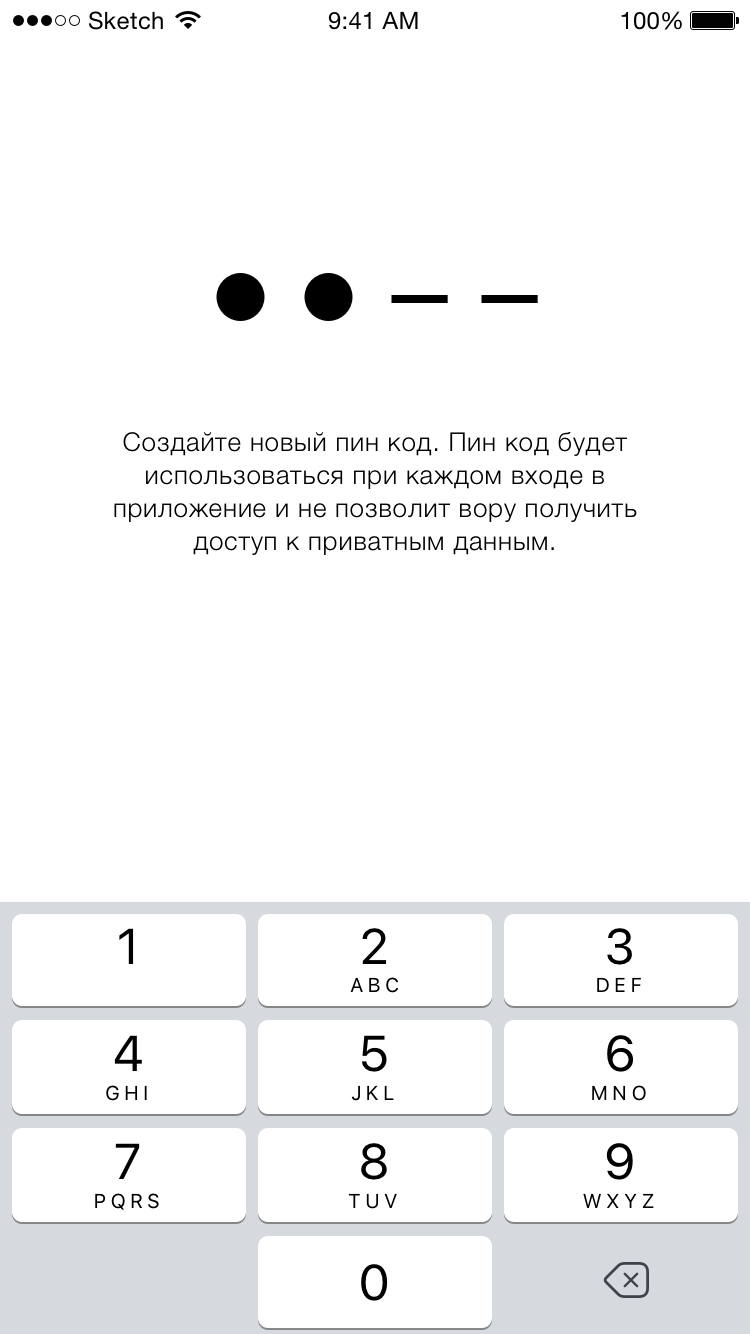
\includegraphics[height=0.25\textheight]{inc/img/ui/pin_code_create.png}
  \captionof{figure}{Экран создания пароля}
  \label{sec:usage:pin:create}
\end{minipage}%
\begin{minipage}{.33\textwidth}
  \centering
  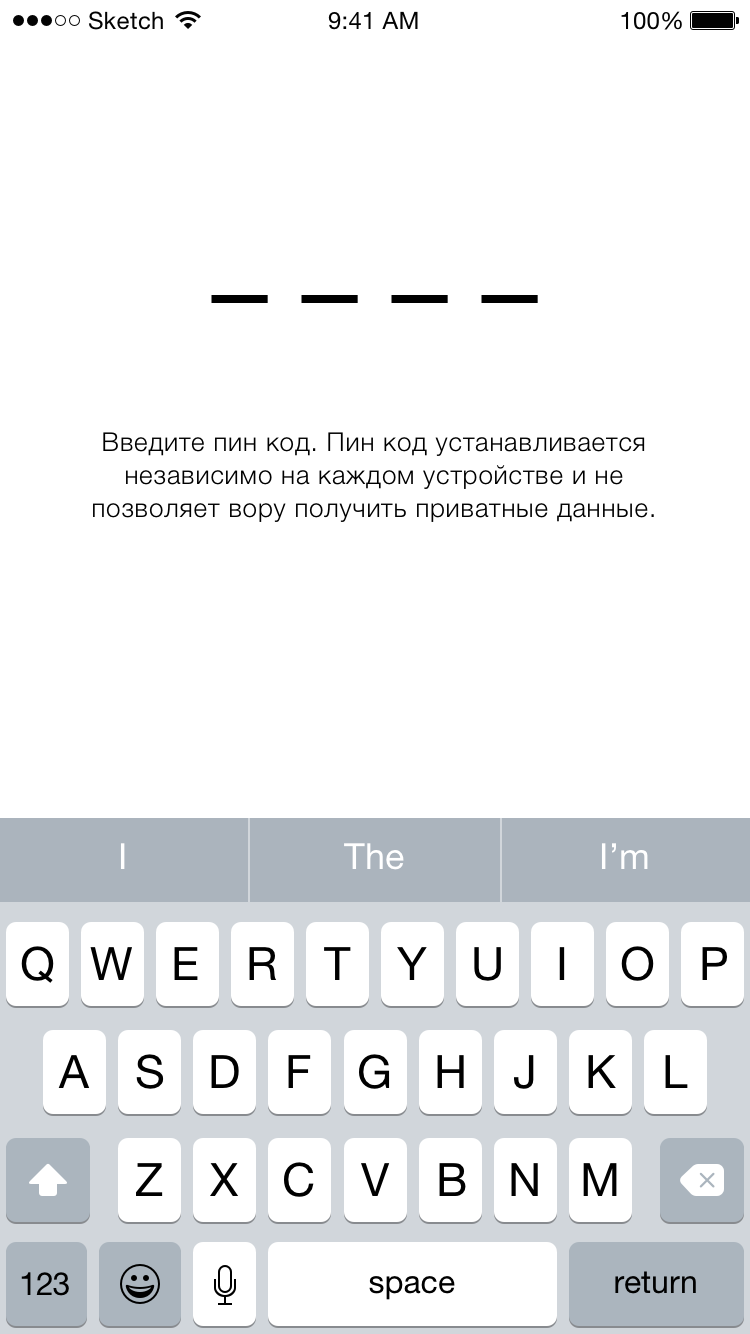
\includegraphics[height=0.25\textheight]{inc/img/ui/pin_code.png}
  \captionof{figure}{Экран ввода пароля}
  \label{sec:usage:pin:enter}
\end{minipage}
\begin{minipage}{.33\textwidth}
  \centering
  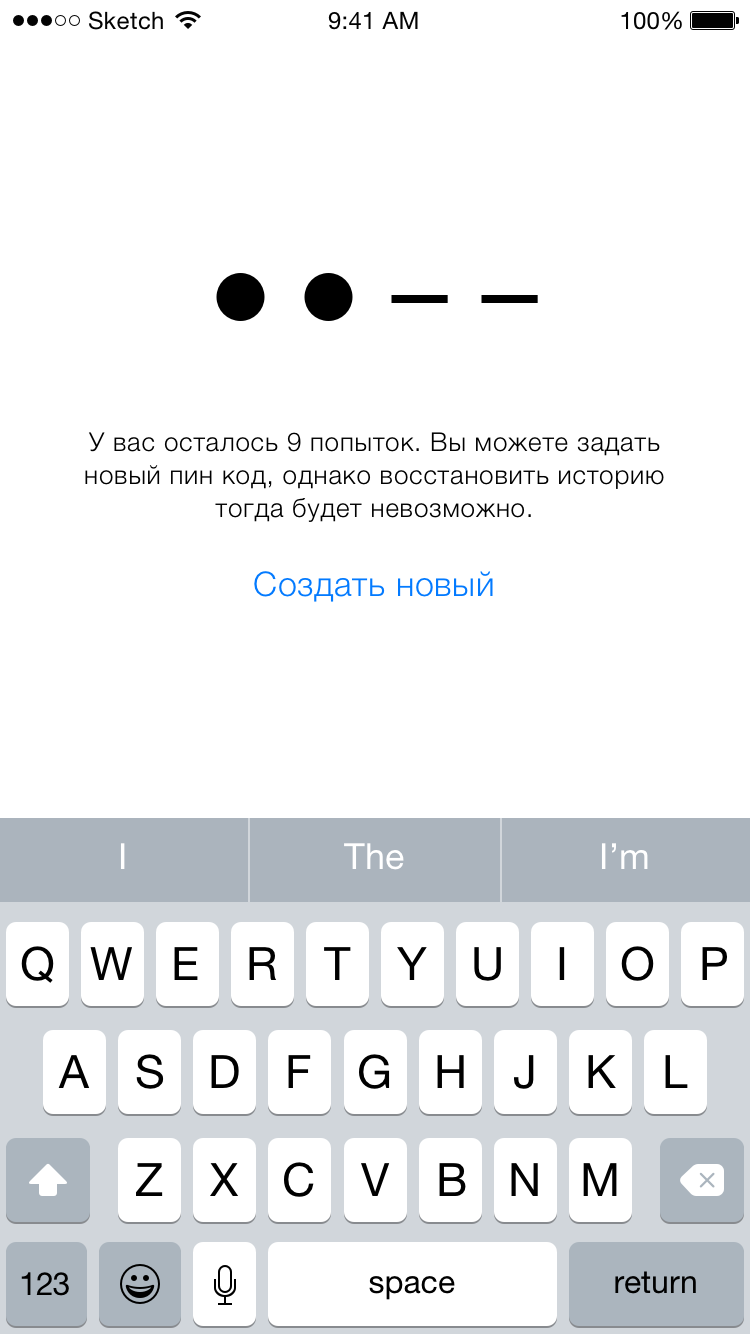
\includegraphics[height=0.25\textheight]{inc/img/ui/pin_core_reset.png}
  \captionof{figure}{Сброс пароля}
  \label{sec:usage:pin:reset}
\end{minipage}
\end{figure}

Сквозвное шифрование не способно защитить пользователя от утери или кражи устройства, что, в свою очередь, ведёт к рискам получения информации не с сервера, но с устройства. Приложение делает всё возможное для повышения безопасности хранимых локально данных и схема активации устройства через пароль приложения является одной из самых эффективных составляющих системы.